\problemname{Full Depth Morning Show}

\illustration{0.3}{radioprize.png}{}

\noindent
All boring tree-shaped lands are alike, while all exciting tree-shaped lands
are exciting in their own special ways. What makes Treeland more exciting than
the other tree-shaped lands are the raddest radio hosts in the local area: Root
and Leaf. Every morning on FM $32.33$ (repeating of course), Root and Leaf of
The Full Depth Morning Show serve up the hottest celebrity gossip and traffic
updates.

The region of Treeland is made of $n$ cities, connected by $n - 1$ roads such
that between every pair of cities there is exactly one simple path. The $i$th
road connects cities $u_i$ and $v_i$, and has a toll of $w_i$.

To reward their loyal listeners, The Full Depth Morning Show is giving away a
number of travel packages! Root and Leaf will choose $n - 1$ lucky residents
from the city that sends them the most fan mail. Each of those residents then
gets a distinct ticket to a different city in Treeland.

Each city in Treeland has its own tax on prizes: $t_i$. Let $d_{u, v}$ be the
sum of the tolls on each road on the only simple path from city $u$ to $v$. For
a trip from city $u$ to city $v$, the cost of that trip is then $(t_u + t_v)
d_{u, v}$.

\begin{figure}[ht!]
\begin{center}
  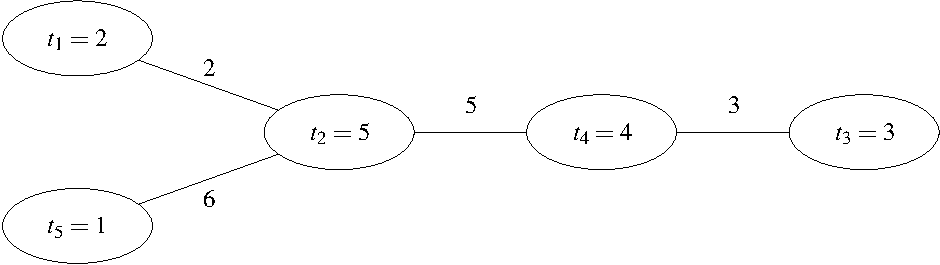
\includegraphics[width=0.7\textwidth]{1}
  \caption{The map of Treeland corresponding to the first sample input.}
  \label{radioprize:1}
\end{center}
\end{figure}

The shock jocks haven't quite thought through how much their prize is worth.
They need to prepare a report to the radio executives, to summarize the
expected costs. For each city that could win the prize, what is the total cost
of purchasing all the tickets?

\section*{Input}

The first line of input is a single integer $n$ ($1 \leq n \leq 100\,000$). The
next line has $n$ space-separated integers $t_i$ ($1\leq t_i \leq 1\,000$), the
tax in each city. The following $n - 1$ lines each have $3$ integers, $u_i,
v_i, w_i$, meaning the $i$th road connects cities $u_i$ and $v_i$ ($1 \le u_i,
v_i \le n$), with a toll of $w_i$ ($1 \leq w_i \leq 1\,000$).

\section*{Output}

Output $n$ lines. On the $i$th line, output a single integer: the cost of
purchasing tickets if city $i$ wins the contest.
